\documentclass[a4paper]{article}

%maximum figure number
\setcounter{totalnumber}{5}

%plus minus
\newcommand{\mypm}{\mathbin{\smash{%
\raisebox{0.35ex}{%
            $\underset{\raisebox{0.5ex}{$\smash -$}}{\smash+}$%
            }%
        }%
    }%
}

%diagbox
\usepackage{diagbox}

%figure inside text
\usepackage{wrapfig}

%layout config
\usepackage{calc}
\setlength\textwidth{7in}
\setlength\textheight{10in}
\setlength\oddsidemargin{(\paperwidth-\textwidth)/2 - 1in}
\setlength\topmargin{(\paperheight-\textheight
-\headheight-\headsep-\footskip)/2 - 1in}

%sinuit
\usepackage{siunitx}
%image insertion
\usepackage{graphicx} %image settings
\DeclareGraphicsExtensions{.pdf,.png,.jpg}

%math
\usepackage{amsmath} %math
%\usepackage{cmbright} %math font

%font
\usepackage{kotex}
\usepackage{fontspec}
\ifx가가
\setmainhangulfont[Ligatures=TeX,
BoldFont={KoPubBatang Medium}]{KoPubBatang Light}
\setsanshangulfont[Ligatures=TeX,
BoldFont={KoPubDotum Medium}]{KoPubDotum Light}
\setmainhanjafont[Ligatures=TeX,
BoldFont={KoPubBatang Medium}]{KoPubBatang Light}
\setsanshanjafont[Ligatures=TeX,
BoldFont={KoPubDotum Medium}]{KoPubDotum Light}
\xetexkofontregime[puncts=prevfont, colons=prevfont, cjksymbols=hangul]{latin}
\fi

%줄간격
\usepackage{setspace}
%\usepackage{indentfirst}
\setstretch{1.2}
\everydisplay{\setstretch{1.2}}

%subfloat
\usepackage{subfig}
% and
\newcommand{\shitn}{&}

\pagestyle{plain}
\title{물리 실험보고서 1}
\author{이한빈, 의예과 2016-13347}

\begin{document}


\numberwithin{equation}{section}
\maketitle

\section{Introduction}
	광전효과는 금속에 빛을 쪼였을 때 전자가 방출되는 현상을 말한다.
	이 때 물체에서 금속이 방출되려면 특정 파장보다 더 짧은 파장의 빛이 쪼여져야만 한다.
	광전효과의 특징에 대한 정밀한 측정을 위해서 다음 그림과 같은 실험장치를 이용한다.
	\begin{figure}[h]
		\centering
		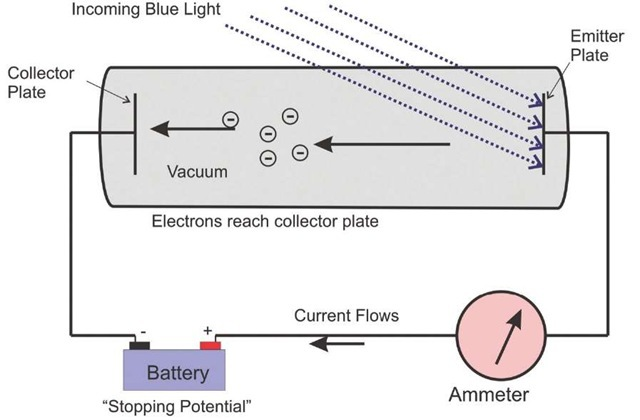
\includegraphics[width=0.4\textwidth]{img/photoex.jpg}
		\label{fig:photoex} \caption{광전효과 실험장치}
	\end{figure}

	이 장치에서는 진공관에 기전력($V$)가 연결되어있으며 전류계를 통해 회로에 흐르는 전류를 측정한다.
	진공관 내부에는 떨어져 있는 양극과 음극이 존재한다.
	실험에서는 양극에 빛을 조사하여 그 때 전류계에 검출되는 광전류를 측정한다.
	전자들이 금속에서 방출되기 위해서는 금속의 종류에만 의존하는 특정한 크기의 에너지를 획득해야만 하는데 이를 일함수($W$)라고 부른다.
	특정 진동수 이상의 빛이 양극에 조사되면 전자들이 운동에너지를 가지고 양극에서 음극으로 이동한다.
	이 때 진공관의 기전력을 걸어주면 양극과 음극 사이에 전자의 운동방향과 반대되는 전위가 형성되어 전자가 음극에 가까워질수록 운동에너지를 잃게된다.
	따라서 $V$을 0에서 서서히 증가시키면 전류계에 흐르는 전류가 0이 되는 순간이 오는데 에너지 보존법칙을 적용하면 이 때 전자가 가지는 운동에너지와 전기적 위치에너지가 같아짐을 알 수 있다.
	따라서 $\frac{1}{2}mv^2 = eV$가 성립한다.
	즉, 전자가 가지는 운동에너지를 측정할 수 있게 되는 것이다.

	이 장치를 통한 실험에서는 빛의 파동성에 위배되는 실험결과들을 얻을 수 있는데 다음과 같다.
	\begin{itemize}
		\item 빛의 세기와 진동수에 따른 전자의 최대 운동에너지 사이에 아무런 연관성이 존재하지 않는다.
		\item 빛의 세기와 무관하게 특정 진동수를 넘는 빛을 조사해야만 전자가 방출된다.
		\item 빛의 세기와 무관하게 빛을 조사하자마자 전자가 방출된다.
	\end{itemize}

	빛의 파동설에 따르면 빛이 가진 에너지는 빛의 세기(진폭)의 제곱에 비례하므로 빛의 세기가 커질수록 전자에게 더 많은 에너지가 전달된다.
	따라서 빛의 세기가 크면 클수록 전자의 최대운동에너지가 커져야하며 빛의 세기가 충분히 커지면 진동수와 무관하게 전자가 방출되어야만 한다.
	그리고 빛의 에너지는 연속적으로 전달되므로 전자가 방출될만큼 충분한 에너지가 공급되기 위해서는 그만큼의 시간이 필요하다.
	그러나 이러한 파동설의 예측들은 실험결과와 위배되므로 파동설로는 이 현상들을 설명할 수 없다.

	아인슈타인은 1905년에 이를 해결하기 위해 빛의 에너지가 덩어리져 전달된다는 광양자설을 주장했는데 이에 따르면 빛은 입자처럼 행동한다.
	광양자설에 따르면 빛의 에너지는 광자라는 빛입자에 의해 전달되는데 각각의 빛 입자는 진도수에 비례하는 에너지를 갖는다.
	구체적으로 $E=hf$만큼의 에너지를 갖는데 여기서 $h$는 플랑크 상수로 미시세계를 기술하는 물리법칙에서 흔히 등장하는 상수다.
	따라서 빛이 조사되었을 때 전자가 얻는 에너지는 전자에 의해 흡수되는 개별 광자의 에너지에 의존하게 되기 때문에 위의 3가지 실험적 사실을 모두 설명할 수 있다.
	광자가 가지는 에너지는 세기와 무관하고 오로지 진동수에만 비례하기 때문에 전자가 획득하는 에너지도 진동수에만 비례하게 된다.
	따라서 전자의 최대운동에너지가 빛의 진동수에만 의존한다는 사실과 특정 진동수 이상의 빛이 조사되었을 때만 전자가 방출되는 현상을 설명할 수 있다.
	그리고 광양자설에 따르면 전자가 에너지를 획득하는 과정은 일정한 크기를 가진 광자를 흡수하는 것이므로 전자가 에너지를 얻어 밖으로 방출되는 사건은 순간적으로 일어나게 되므로 세 번째 실험사실과도 잘 일치한다.

	마지막으로 아인슈타인이 제시한 $E = hf$라는 공식을 이용하면 이 실험에 대한 정량적인 계산을 할 수 있다.
	회로에 전압 $V$가 걸려있을 때 전자가 음극에 도달했을 때 최종적으로 가지는 운동에너지는 광자가 전달해준 에너지에서 양극을 이루는 금속의 일함수와 양극과 음극사이의 전위차를 빼준 것이 된다.
	\begin{equation}
		\frac{1}{2}mv^2 = hf - W - eV
	\end{equation}
	
	따라서 위 식이 성립하는데 V의 값을 조절하여 광전류가 0이 되도록 하는 최소의 전압 $V_0$를 택하면 그 때 음극에서 전자의 운동에너지가 0이 되어 양극에서 방출된 전자가 더 이상 음극에 도달하지 못하고 따라서 검류계에 측정되는 전류가 0이 되는 것임을 알 수 있다.
	\begin{equation}
		0 = \frac{1}{2}mv^2 = hf - W - eV_0
		\label{eq:core}
	\end{equation}

	즉, $eV_0$와 $f$에 대한 그래프를 그리면 그 그래프는 일차함수가 되고 그 일차함수의 기울기가 플랑크 상수 $h$가 됨을 알 수 있다.
	이로부터 광전효과를 이용하면 플랑크 상수를 측정할 수 있다.

	본 실험의 플랑크 상수 측정 장치는 빛의 세기를 편광판을 이용해 조절한다.
	편광된 빛을 사용한 실험장치[2]는 빛의 전기장축과 편광판이 이루는 각도가 $\theta$로 주어졌을 때 다음 식을 만족한다.
	\begin{equation}
		I = I_{0}\cos{\theta}^{2}
		\label{eq:polar}
	\end{equation}
	따라서 $\theta$가 \ang{0}과 \ang{90}사이에서 바뀌면 $\theta$가 커질수록 빛의 세기가 약해짐을 알 수 있다.

	본 실험에서는 앞서 기술된 내용들을 바탕으로 플랑크 상수를 측정하고 광전효과의 실험적 사실들을 확인하며 이로부터 빛의 입자성에 대해서 알아본다.

\section{Method}
	준비물 : 플랑크 상수 측정 기기
	\subsection{플랑크 상수 측정}
		1. 편광판 각도를 \ang{0}, 광전류가 최대가 되도록 저항값을 조절하고 영점을 맞춘 후 색깔을 Red로 놓는다. \\
		2. 저지전압을 조절해 광전류가 0이 되도록 맞춘 후 그 떄의 저지전압을 기록한다. \\
		3. 색깔을 Green, Orange, Blue, Purple에 대해 반복한다.

	\subsection{빛의 세기와 광전류의 관계}
		1. 편광판 각도를 \ang{0}, 광전류가 최대가 되도록 저항값을 조절하고 영점을 맞춘 후에 색깔을 Red로 놓는다. \\
		2. 편광판 각도을 \ang{0}부터 \ang{5}씩 증가시키며 광전류를 측정하고 기록한다. \\
		3. 색깔을 Green, Orange, Blue, Purple에 대해 반복한다.

	\subsection{빛의 세기와 저지전압의 관계}
		1. 편광판 각도를 \ang{0}, 광전류가 최대가 되도록 저항값을 조절하고 영점을 맞춘 후에 색깔을 Blue로 놓는다. \\
		2. 그 때 저지전압을 조절하여 광전류가 0이 되록한다. \\
		3. 편광판 각도를 \ang{5}씩 증가시키며 위의 과정을 반복한다. 

\section{Result}
	\subsection{측정 장비 스펙}
		플랑크 상수 측정기기의 광원 파장은 다음과 같다[2].
		\begin{figure}[h] 
		\centering
			\begin{tabular}{|c|c|c|c|c|c|}
				\hline 
				색깔 & Red & Green & Orange & Blue & Purple \\
				\hline
				파장(\si{nm}) & 685 & 640 & 520 & 465 & 420 \\ 
				\hline
			\end{tabular}
			\caption{플랑크 상수 측정기기의 색깔에 따른 파장}
		\end{figure}

	\subsection{플랑크 상수 측정}
		\begin{figure}[h]
		\centering	
			\subfloat[편광판의 각도와 색깔에 따른 저지전압]{
				\begin{tabular}{|c|c|c|c|c|c|}
				\hline
				\diagbox{$\theta$}{Color} & Red & Orange & Green & Blue & Purple \\
				\hline
				\ang{0} & 0.1 & 0.17 & 0.42 & 0.68 & 0.92 \\
				\hline
				\ang{30} & 0.1 & 0.17 & 0.42 & 0.68 & 0.92 \\
				\hline
				\ang{60} & 0.1 & 0.17 & 0.42 & 0.68 & 0.92 \\
				\hline
			\end{tabular}
			}
			//
			\subfloat[V = $\frac{hc}{e} \frac{1}{\lambda} - \frac{W}{e}의 그래프$]{
				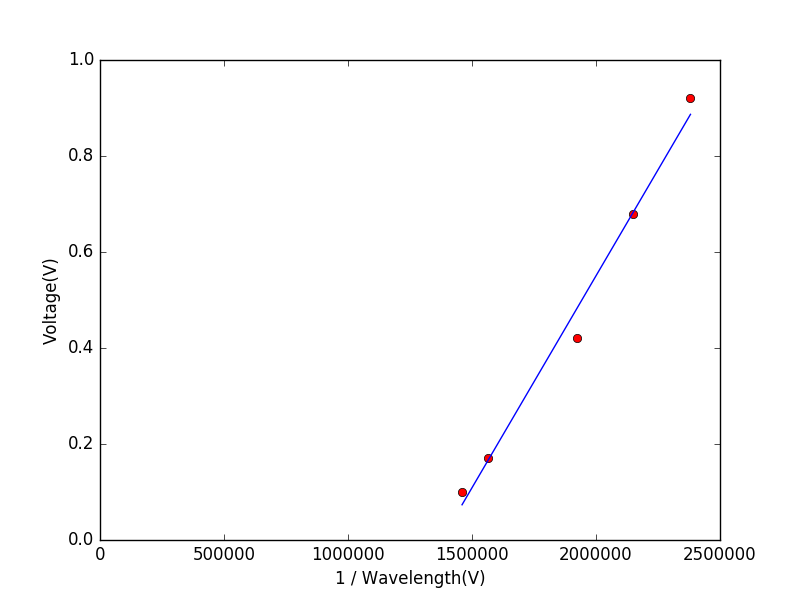
\includegraphics[width=0.5\textwidth]{img/figure_1.png}
			}

		\end{figure}
		$\frac{hc}{e} = 8.83 \times 10^{-7}$, $\frac{W}{e} = -1.215$로 측정되었다.
		$R^2 = 0.987$이다. 
		따라서 플랑크 상수 $h = 4.716 \times 10 ^{-34} \si{m^2 \cdot kg /s}$이다.
		Fitting은 Scipy로 이루어졌다.


	\subsection{빛의 세기와 광전류의 관계}
		\begin{figure}[h]
		\centering
			\begin{tabular}{|c|c|c|c|c|c|c|c|c|c|c|c|c|c|c|c|c|c|c|c|}
			\hline
			\diagbox{색깔}{각도($^{\circ}$)} & 0 & 5 & 10 & 15 & 20 & 25 & 30 & 35 & 40 & 45 & 50 & 55 & 60 & 65 & 70 & 75 & 80 & 85 & 90 \\
			\hline
			Red & 3 & & & & & & 2 & & & 1 & & & & & 0 & & & & \\
			\hline
			Yellow & 7 & & & 6 & & & 5 & & 4 & 3 & & 2 & & 1 & 0 & & & & \\
			\hline
			Green & 34 & & 33 & & 30 & & 26 & 23 & 21 & 18 & 15 & 12 & 9 & 7 & 4 & 3 & 1 & 0 & \\
			\hline
			Blue & 103 & & 101 & 98 & 95 & 90 & 83 & 75 & 68 & 60 & 50 & 43 & 31 &25 & 17 & 10 & 6 & 1& 0 \\
			\hline 
			Purple & 175 & 171 & 166 & 160 & 150 & 140 & 127 & 112 & 98 & 83 & 68 & 53 & 40 & 28 & 17 & 9 & 4 & 2 \\
			\hline
		\end{tabular}
		\caption{빛의 세기와 광전류의 관계. 단위는 \si{\mu A}}
	\end{figure}
	값이 변하지 않은 칸들은 공란으로 처리하였다. 
	실험된 모든 파장에 대해서 빛의 세기가 작아질수록 광전류의 크기도 작아지는 것을 관찰할 수 있다.

	\subsection{빛의 세기와 저지전압과의 관계}
		\begin{figure}[h]
			\begin{tabular}{|c|c|c|c|c|c|c|c|c|c|c|c|c|c|c|c|c|c|}
			\hline
			각도($^{\circ}$) & 0 & 5 & 10 & 15 & 20 & 25 & 30 & 35 & 40 & 45 & 50 & 55 & 60 & 65 \\
			\hline
			저지전압(\si{V}) & 0.72 & 0.72 & 0.72 & 0.72 & 0.72 & 0.72 & 0.72 & 0.72 & 0.72 & 0.72 & 0.72 & 0.72 & 0.72 & 0.72 \\
			\hline
			각도($^{\circ}$) & 70 & 75 & 80 & 85 & 90 \\
			\hline
			저지전압(\si{V}) & 0.72 & 0.72 & 0.72 & 0.72 & 0.72 \\	
			\hline
			\end{tabular}
			\caption{빛이 세기와 광전류의 관계}
		\end{figure}
		빛의 세기가 달라지더라도 저지전압이 바뀌지 않음을 알 수 있다.

	\section{Conclusion}
	플랑크 상수를 구하기 위해서 피팅한 결과의 $R^2$값은 1에 매우 가깝게 나타나 이론으로 예측된 일차식과 잘 일치함을 알 수 있다.
	또한 측정된 플랑크 상수는 $4.716 \times 10^{-34} \si{m^2 \cdot kg /s}$로 실제값인 $6.626 \times 10^{-34} \si{m^2 \cdot kg /s}$과 28.8\%의 차이를 보였다. 

	오차의 원인으로 플랑크 상수 측정기기의 유효숫자 자릿수와 최종 자리수 근처에서 숫자가 계속 요동치던 현상을 생각할 수 있다.
	플랑크 상수 측정 장치의 전압계는 V단위로 소숫점 둘쨋자리까지 측정할 수 있었고 측정된 전압은 최대 소숫점 첫째짜리까지 존재하므로 유효숫자와 최종자릿수 근처에서의 요동은 최대 5\%까지의 오차 밖에 설명하지 못한다.

	그 외에 광전류 값이 0을 나타내는 저지전압이 하나의 값으로 나타나지 않고 구간을 가지고 나타난 것이 하나의 원인으로 추측된다.
	하지만 실험 당시에 광전류 값이 0이 되는 저지전압의 구간을 기록하지 못했으므로 본 보고서에서는 정량적인 논의를 하지 못했다.

	빛이 입자성을 가지고 있는 지에 대해서도 알아보았다.
	두 번째 실험에서 편광판의 각도가 커질수록 빛의 세기가 약해진다(식(\ref{eq:polar}).
	따라서 실험결과는 빛의 세기가 강할수록 광전류가 커진다는 것을 얘기하고 있다.
	빛의 입자설에 따르면 전자와 광자는 1:1로 흡수하여 광전자를 생산한다.
	그런데 입자설에 따르면 빛의 세기는 광양자의 갯수에 비례하므로 광양자설은 두 번째 실험결과와 부합한다.

	Intro에서 밝혔듯이 빛의 최대 운동에너지는 실험 3에서처럼 저지전압을 이용해 알아낼 수 있다.
	그런데 실험결과는 저지전압과 빛의 세기가 무관하다는 것을 보여주고 있으므로 역시 빛의 입자설과 부합하는 결과임을 알 수 있다. 
	

\section{Reference 및 부록}
	[1] Halliday, D., Resnick, R., \& Walker, J. (2014). {\it{}Principles of Physics} (10th ed., Vol. 2). Hoboken, NJ: Wiley. \\
	{[2]} (주)서울과학기기 http://www.physicspro.co.kr/
\end{document} 

%실험에서 개선할 점 등 피피티에서 봤던 거 모두 적어서 처리합시다